\chapter{Non-relativistic Quantum Field Theory}
A general non-relativistic field has the Lagrangian\footnote{The repeated indices are automatically summed.}
\begin{equation}
	\mathcal L = \bar\psi_a(x) (i\delta_{ab}\partial_t-\hat H_{ab})\psi_b(x) + \mathcal{V}_{\mathrm{int}}
\end{equation}
where the field operator $\psi$ can be bosonic or fermionic, which is denoted by a number $\zeta=\pm 1$, and $\mathcal{V}_{\mathrm{int}}$ is the interaction Lagrangian.
A general interaction has the form
\begin{equation}
	\mathcal{V}_{\mathrm{int}} = \bar\psi_{a}(x_1)\bar\psi_{b}(x_2) V_{ab}(x_1,x_2) \psi_{b}(x_2)\psi_{a}(x_1).
\end{equation}
Note that the classical equation of motion for the free field is
\begin{equation}
\begin{aligned}
	0 &= \partial_\mu \frac{\partial \mathcal L}{\partial(\partial_\mu \bar\psi_a(x))} - \frac{\partial \mathcal L}{\partial\bar{\psi}_a(x)} \\
	&= - i\partial_t \phi_a(x) + \hat H_{ab}\phi_b(x),
\end{aligned}
\end{equation}
which satisfies the Schr\"{o}dinger equation.

We are mostly work with finite system size $L^d$ with UV cutoff $\Lambda = \frac{2\pi}{a}$,\footnote{We can regard $a$ as the lattice spacing, and assume $L = Na$.} in which case the spatial Fourier transformation is
\begin{eqnarray}
	\tilde{\psi}_a(k) &=& \int_{L^d} d^dx e^{-i k \cdot x}\psi(k), \\
	\psi_a(x) &=& \frac{1}{L^d}\sum_{k} e^{i k \cdot x}\tilde{\psi}(k).
\end{eqnarray}
Note that for finite size, the momentum is discretized: 
\begin{equation}
	k_i = \frac{2\pi}{L} n_i,\ n_i = -N,\cdots,N.
\end{equation}
By default, we take the thermodynamic limit.
The summation is approximated by the integration:
\begin{equation}
	\frac{1}{L^d}\sum_k \longrightarrow \int_{|k|<\Lambda} \frac{d^dk}{(2\pi)^d}.
\end{equation}

\section{Finite Temperature Field Theory}
The original real-time partition function is defined as\footnote{As with the relativistic case, we introduce an auxiliary source $J$, which is bosonic/fermionic if the field $\psi$ is bosonic/fermionic.
}
\begin{equation}
	Z[J] = \int D[\bar\psi,\psi] \exp\left\{i\int dt \int d^dx \left[\mathcal{L}+\bar{J}_a(x)\psi_a(x)+\bar{\psi}_a(x)J_a(x)\right]\right\}.
\end{equation}
For finite-temperature field theory, after making the wick rotation $t \rightarrow -i\tau$, the partition function for a generic non-relativistic lattice theory is:
\begin{equation}
	Z[J] = \int D[\bar\psi,\psi] e^{-S[\bar\psi,\psi]+\bar{J}\cdot\psi+\bar{\psi}\cdot J},
\end{equation}
where the action is
\begin{equation}
	S = \int_0^\beta d\tau \int d^dx \left[\bar\psi_a(x) (\delta_{ab}\partial_\tau+\hat H_{ab})\psi_b(x) + \mathcal{V}_{\mathrm{int}}\right].
\end{equation}

\begin{framedrmk}[Temporal Fourier Transformation]
The Fourier transformation on the imaginary time domain is defined as:
\begin{eqnarray}
	\tilde\psi(\omega_n) &=& \int_0^\beta d\tau e^{i\omega_n\tau} \psi(\tau),\\ 
	\psi(\tau) &=& \frac{1}{\beta}\sum_{\omega_n} e^{-i\omega_n\tau} \tilde\psi(\omega_n).
\end{eqnarray}
Under such convention, in the thermodynamic limit and zero-temperature limit, the spatial-temporal Fourier transformation agrees with the relativistic case (up to a Wick rotation).
\end{framedrmk}


\subsection{Free Field Theory}
We first consider the action of free field
\begin{equation}
	S_0 = \int_0^\beta d\tau \int d^dx\ \bar\psi_a(x) (\delta_{ab}\partial_\tau+\hat H_{ab})\psi_b(x).
\end{equation}
The Fourier transformation
\begin{equation}
	S_0 = \frac{1}{\beta}\sum_{\omega_n} \int_{\Lambda} \frac{d^dk}{(2\pi)^d}
	\tilde{\bar{\psi}}_a(k,\omega_n)\left[-i\omega_n + \tilde{H}_{ab}(k)\right]\tilde{\psi}_b(k,\omega_n).
\end{equation}
The partition function with source is
\begin{equation}
	\frac{Z_0[J]}{Z_0[0]} = \exp\left[-\frac{1}{\beta}\sum_{\omega_n} \int_{\Lambda} \frac{d^dk}{(2\pi)^d}\tilde{\bar J}_a(k,\omega_n) \tilde{G}_{ab}(k,\omega_n) \tilde{J}_b(k,\omega_n) \right],
\end{equation}
where the Green's function is
\begin{equation}
	\tilde{G}_{ab}(k,\omega_n) = \left[\frac{1}{i\omega_n - \tilde{H}(k)}\right]_{ab}.
\end{equation}

\begin{framedrmk}[Obtaining the Partition Function]
Unlike the relativistic case, the value of the value of partition function without source $Z_0[0]$ is related to the free energy.
We can express it formally as
\begin{equation*}
	Z_0[0]= \left[\det (-G_{ab})^{-1}\right]^{-\zeta}.
\end{equation*}
To get the correct dimensionality, we set the determinant as
\begin{equation*}
	Z_0[0] \equiv \prod_{k,\omega_n}\left\{\beta \det\left[-i\omega_n+\tilde{H}(k)\right]\right\}^{-\zeta}.
\end{equation*}
Thus the free energy is
\begin{equation}
	F = -\frac{1}{\beta} \ln Z_0
	= \zeta \sum_{k,\omega_n} \ln\left\{\beta\det\left[-i\omega_n+\tilde{H}(k)\right]\right\}.
\end{equation}
\end{framedrmk}

\begin{framedrmk}[Matsubara Summation]
Now consider the summation on Matsubara frequency:
\begin{equation}
	\sum_{\omega_n} f(\omega_n) = 
	\begin{cases}
		\sum_n f(\frac{2n\pi}{\beta}) & \mathrm{bosonic} \\
		\sum_n f(\frac{(2n+1)\pi}{\beta}) & \mathrm{fermionic}
	\end{cases}.
\end{equation}
The frequency is capture by the singularities of the density function of the states:
\begin{equation}
	\rho(z) = \begin{cases}
		\frac{1}{\exp(\beta z)-1} & \mathrm{bosonic} \\
		\frac{1}{\exp(\beta z)+1} & \mathrm{fermionic}
	\end{cases}.
\end{equation}
The residue on imaginary frequency $i\omega_n$ is alway $\frac{1}{\beta}$. In this way, the summation is:
\begin{equation}
	\frac{1}{\beta}\sum_{\omega_n} f(i\omega_n) 
	= \frac{1}{2\pi i} \oint \rho(z)f(z)
	= -\sum_{k} \mathrm{Res}\ \rho(z)f(z)|_{z=z_k}.
\end{equation}
\end{framedrmk}

\begin{framedexpl}[Summation of Green's function]
Consider the frequency summation for the correlation function:
\begin{equation*}
	\frac{1}{\beta}\sum_{\omega_n} \tilde{G}_0(k) 
	= \frac{1}{\beta}\sum_{\omega_n}\frac{1}{i\omega_n-E_{p}}
	= -\mathrm{Res} \left. \frac{\rho(z)}{z-E_{p}}\right|_{z=E_{p}}
	= \rho(E_{p}).
\end{equation*}
\end{framedexpl}

\begin{framedexpl}[Summation of Green's function]
Consider the frequency summation for the correlation function:
\begin{equation*}
	\sum_{\omega_n} \langle\bar\psi_{\vec p,\omega_n}\psi_{\vec p, \omega_n}\rangle = \frac{1}{\beta}\sum_{\omega_n}\frac{1}{-i\omega_n+\epsilon_{\vec p}}
	= \mathrm{Res} \left. \frac{\rho(z)}{z-\epsilon_{\vec p}}\right|_{z-\epsilon_{\vec p}}
	= \rho(\epsilon_{\vec p}).
\end{equation*}
\end{framedexpl}
\begin{framedexpl}[Free Energy Summation]
Consider the free energy
\begin{equation*}
	F = -\frac{1}{\beta}\ln Z 
	= -\frac{1}{\beta}\sum_{\omega_n}\ln[\beta(-i\omega_n+E_{\vec p})]
	= \frac{1}{2\pi i} \oint dz \rho(z)\ln[\beta(\xi - z)].
\end{equation*}
To calculate the summation, we consider the line integral along the loop:
\begin{equation*}
	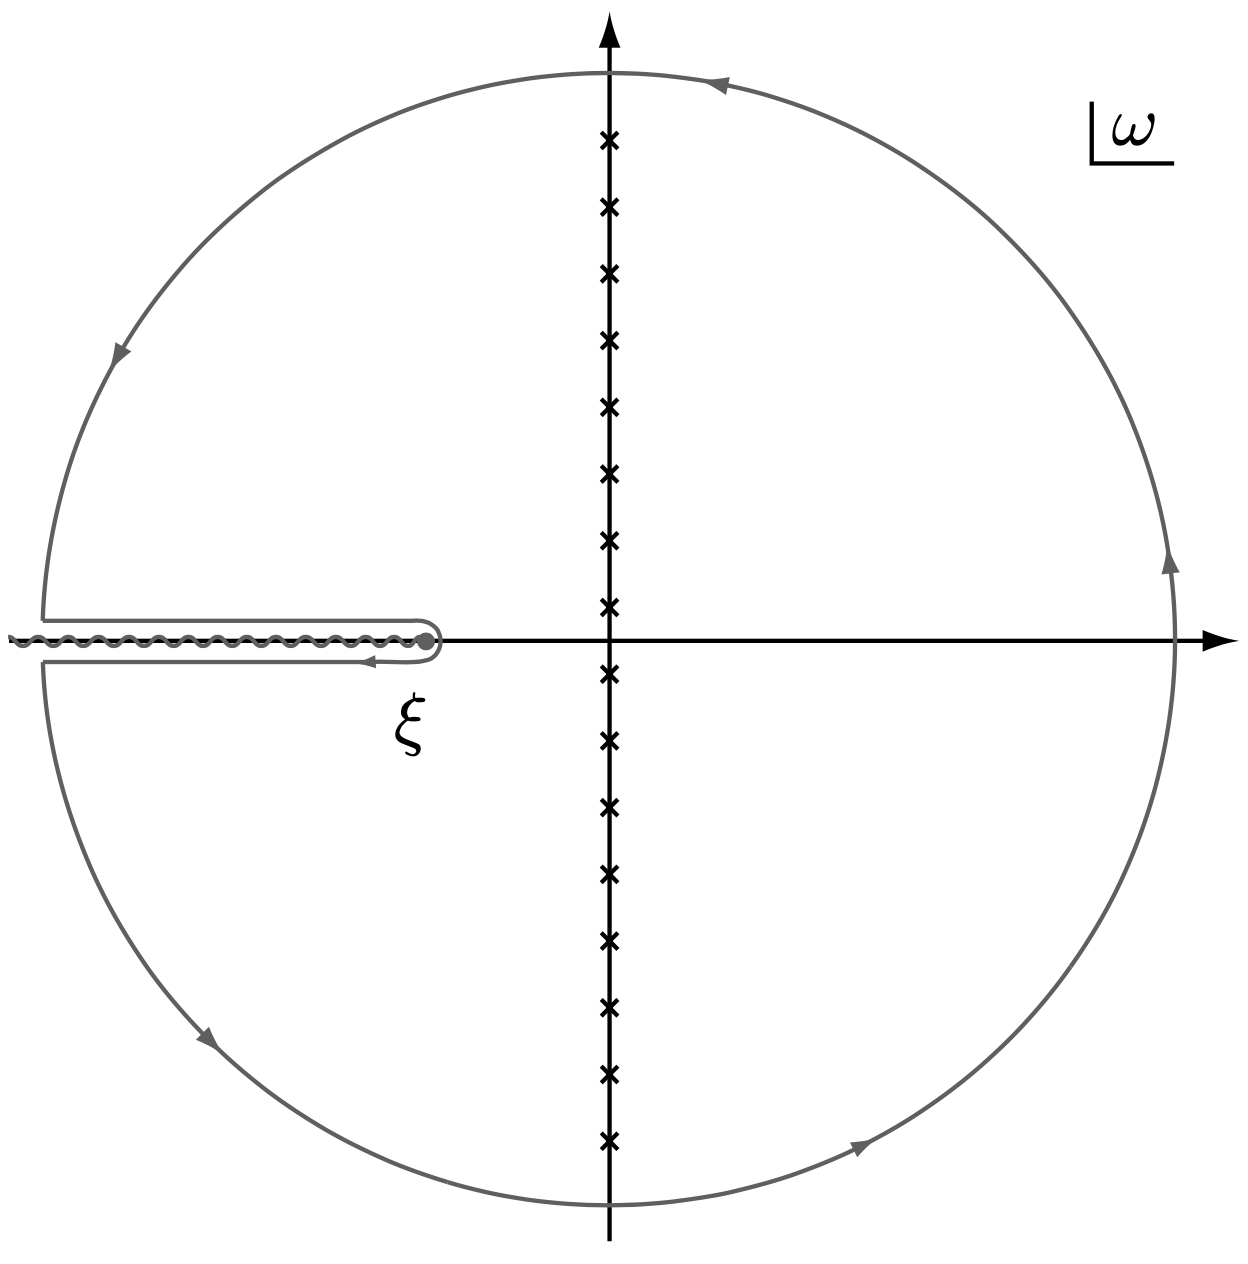
\includegraphics[width=0.3\linewidth]{pics/FqSum.png}
\end{equation*}
The free energy is
\begin{equation*}
\begin{aligned}
	F &= \frac{1}{2\pi i}\int_{-\infty}^\infty dx \rho(x)\ln\left(\frac{\xi-x-i\epsilon}{\xi-x+i\epsilon}\right) \\
	&= \frac{-\zeta}{2\pi i\beta} \int_{-\infty}^{\infty}dx \ln(1-\zeta e^{-\beta z})\left(\frac{1}{x+i\epsilon-\xi}-\frac{1}{x-i\epsilon-\xi}\right),
\end{aligned}
\end{equation*}
where we integrate the expression by part, noticing that
\begin{equation}
	\frac{d}{dz} \frac{\zeta}{\beta} \ln(1-\zeta e^{-\beta z}) = \frac{1}{e^{\beta z}-\zeta} = \rho(z)
\end{equation}
Using the identity
\begin{equation*}
	\lim_{\epsilon\rightarrow 0^+} \frac{1}{x+i\epsilon} = -i\pi\delta(x) + \mathcal{P}\frac{1}{x},
\end{equation*}
the above expression can be simplified to
\begin{equation}
	F = \frac{\zeta}{\beta} \ln(1-\zeta e^{-\beta\zeta}).
\end{equation}
\end{framedexpl}









